
\section{Processi di supporto}\label{PS}

	\subsection{Documentazione}\label{PS:Documentazione}

		\subsubsection{Implementazione}\label{PS:Documentazione:Implementazione}

			\paragraph{Template}\label{PS:Documentazione:Implementazione:Template}
			Prima di iniziare a redigere i documenti, abbiamo creato un \gloss{template} per \LaTeX \ (\S\ref{LaTeX}) contenente tutte le impostazioni grafiche
			condivise tra questi, per sfruttare il riutilizzo del codice e semplificare enormemente la manutenzione dei sorgenti.\par
			Nello specifico, è presente un file per ognuna delle seguenti utilità:
			\begin{itemize}
				\item \gloss{Layout} delle pagine
				\item \gloss{Macro} personalizzate volte a semplificare l'utilizzo di strutture o comandi ricorrenti
				\item Codice per la generazione della prima pagina
					(struttura definita in \S\ref{PS:Documentazione:Struttura:Frontespizio})
				\item Diario delle modifiche
			\end{itemize}

			\paragraph{Ciclo di vita dei documenti}\label{PS:Documentazione:Implementazione:CicloVita}
			Durante il suo ciclo di vita, ogni documento potrà trovarsi in una delle seguenti fasi:
			\begin{itemize}
				\item \textbf{Redazione}: fase che inizia con la creazione del documento e dura fino alla sua ultima approvazione.
					Il \Res\ assegna ai \gloss{redattori} le varie sezioni di ogni documento da redigere, i quali aggiorneranno la versione nel diario delle modifiche
					come normato in \S\ref{Versionamento}.
				\item \textbf{Verifica}: il documento entra in questa fase nel momento in cui i Redattori hanno terminato la stesura del lavoro loro assegnato, segnalandolo al \Res, che a sua volta assegnerà ai Verificatori la verifica della qualità del prodotto, secondo quanto riportato nelle norme di verifica. Essi potranno approvare il documento oppure notificare il \Res\ su eventuali errori o incongruenze emerse durante la fase di verifica, che provvederà a riassegnare il lavoro.
				\item \textbf{Approvazione}: fase che inizia dall'accettazione del documento da parte dei Verificatori nella fase di verifica. Spetta al \Res\
					l'approvazione ufficiale del documento, seguita dal rilascio di una \gloss{major release}.
			\end{itemize}

		\subsubsection{Struttura}\label{PS:Documentazione:Struttura}

			\paragraph{Frontespizio}\label{PS:Documentazione:Struttura:Frontespizio}
			La prima pagina di ogni documento, sarà caratterizzata da:
			\begin{itemize}
				\item Logo e nome del gruppo
				\item Titolo del documento
				\item Informazioni sul documento:
					\begin{itemize}
						\item Versione documento
						\item Data di creazione e ultima modifica
						\item Nominativo dei Redattori
						\item Nominativo dei Verificatori
						\item Nominativo del \Res
						\item Destinazione d'uso
						\item Destinatari del documento
						\item Contatto del gruppo
					\end{itemize}
				\item Breve descrizione del documento
			\end{itemize}

			\paragraph{Storico delle versioni}\label{PS:Documentazione:Struttura:StoricoVersioni}
			La pagina che segue il frontespizio contiene lo storico delle versioni del documento, in cui ogni aggiunta o modifica significativa ha
			comportato un incremento di versione. Ogni riga contiene, a partire da sinistra:
			\begin{itemize}
				\item Il numero della versione nel formato espresso in \S\ref{Versionamento}
				\item Una breve descrizione delle modifiche apportate
				\item Il ruolo dell'autore che ha apportato la modifica
				\item Il nominativo dell'autore
				\item La data di modifica
			\end{itemize}
			La chiave primaria della tabella è il numero di versione ordinata in senso decrescente, in modo che la versione più vecchia sia
			l'ultima riga della tabella.

			\paragraph{Indice}\label{PS:Documentazione:Struttura:Indice}
			In ogni documento, esclusi i verbali, è presente un indice contenente tutte le sezioni, sottosezioni e paragrafi. I numeri di sezioni, sottosezioni,
			e paragrafi sottostanti saranno separati da un punto (e.g. 1.4.1).\par
			Saranno eventualmente presenti un indice delle
			figure e un indice delle tabelle, assenti in caso non ci siano tabelle o figure nel documento.\par
			I valori degli indici partono da 1.

			\paragraph{Contenuto}\label{PS:Documentazione:Struttura:Contenuto}
			La struttura di ogni pagina presenta:
			\begin{itemize}
				\item Intestazione con:
				\begin{itemize}
					\item A sinistra, logo di \gruppo
					\item A destra, nome del capitolato e documento corrente
				\end{itemize}
				\item Piè di pagina con:
				\begin{itemize}
					\item A sinistra, nome e mail di riferimento del gruppo
					\item A destra, numero della pagina corrente
				\end{itemize}
			\end{itemize}


		\subsubsection{Design}\label{PS:Documentazione:Design}

			\paragraph{Norme tipografiche}\label{PS:Documentazione:Design:NormeT}
			Le norme tipografiche qui di seguito elencate sono state decise in modo che ognuno di noi concorra a mantenere una forma coerente e univoca
			per tutti i documenti redatti.
			
			\subparagraph{Stile redazionale}
			Lo stile redazionale dei vari documenti sarà prevalentemente personale, in prima persona, per rendere chiaro il soggetto delle frasi.

			\subparagraph{Stile del testo}\label{PS:Documentazione:Design:NormeT:StileTesto}
			\begin{itemize}
				\item \textbf{Corsivo}: solo per i nomi dei documenti citati.
				\item \textbf{Maiuscolo}: la prima lettera per
				\begin{itemize}
					\item Tutte le parole appartenenti ai nomi dei documenti tranne gli articoli
					\item Nomi dei ruoli
					\item Prima parola degli elenchi puntati
				\end{itemize}
			\end{itemize}

			\subparagraph{Elenchi puntati}\label{PS:Documentazione:Design:NormeT:ElenchiPuntati}
			\begin{itemize}
				\item \textbf{Simboli di livello}: un pallino nero per il primo livello, un trattino per il secondo livello.
				\item \textbf{Punteggiatura}: nessuna punteggiatura alla fine di una frase, tranne nel caso in cui sia presente una descrizione.
					In quel caso la descrizione è preceduta dai due punti ``:'' e termina con un punto ``.''.
				\item \textbf{Grassetto}: solo se è presente una descrizione, allora sono in grassetto tutte le parole prima dei due punti ``:''.
			\end{itemize}

			\subparagraph{Altri formati testuali comuni} \label{PS:Documentazione:Design:NormeT:AltriFormati}
			\begin{itemize}
				\item \textbf{Orari}: \texttt{HH:MM} secondo la norma ISO 8601\footnote{Riferirsi alla voce ``ISO 8601'' in \S\ref{rifnorma}}
				nel formato 24 ore dove:
				\begin{itemize}
					\item \texttt{HH} indica le ore, da 00 a 23
					\item \texttt{MM} i minuti, da 00 a 59
				\end{itemize}
				\item \textbf{Date}: \texttt{YYYY-MM-DD} formato adottato in Europa dove:
				\begin{itemize}
					\item \texttt{YYYY} l'anno
					\item \texttt{MM} il mese, da 01 a 12
					\item \texttt{DD} il numero del giorno, da 01 a 31
				\end{itemize}
				\item \textbf{Nota a piè di pagina}: serve ad inserire elementi aggiuntivi, come osservazioni o riferimenti a parti interne al documento, utili alla comprensione del testo,
				ma se inseriti all'interno del discorso, ne interromperebbero la lettura, rendendola meno scorrevole.
			\end{itemize}


			\paragraph{Elementi grafici}

			\subparagraph{Figure}
			Ogni immagine inserita nei documenti deve sempre essere centrata rispetto al foglio e adeguatamente separata dal testo. Deve inoltre essere
			accompagnata da una breve \gloss{caption} che permetta al lettore di capire esattamente che cosa sta guardando.\\
			È presente nell'indice l'elenco delle figure che raccoglie la lista di tutte le immagini presenti.

			\subparagraph{Tabelle}\label{StrumentiDiSupportoTabelle}
			Come per le figure, ogni tabella sarà accompagnata da una caption e sarà della dimensione del testo, o se più piccola, centrata.
			Tutte le tabelle saranno raccolte nell'elenco delle tabelle.\par
			Saranno presenti due tipologie di tabelle:
			\begin{itemize}
				\item \textbf{Semplici}: tabelle standard senza uno stile particolare, in cui le celle sono separate da bordi neri (evitare, ove non risulta necessario,
					le righe verticali).
				\item \textbf{Complesse}: tabelle con un'alternanza di colori tra le righe delle celle (grigio e bianco) e senza bordi verticali.
					Le celle sono separate orizzontalmente da una corretta spaziatura e allineamento e verticalmente dall'alternanza dei due colori.
					La riga dell'\gloss{header} può essere bianca o di un grigio più scuro in base al contesto, con il testo che può essere in grassetto.
			\end{itemize}


		\subsubsection{Produzione}

			\paragraph{Suddivisione dei documenti}\label{SuddivisioneDeiDocumenti}

			\subparagraph{Documenti interni}
			Le \NdP\ e lo \SdF\ sono documenti interni, consultabili solo dal team e dal committente, per motivi didattici.

			\subparagraph{Documenti esterni}
			Sono considerati esterni, invece, il \PdP, il \PdQ\, il \Gl\ e l'\AdR\ che, al contrario dei precedenti, vengono consegnati al proponente.

			% Questi documenti sono ufficiali e approvati direttamente dal \Res\ e comprendono, per esempio: \PdP, \PdQ\ e \AdR. Si chiamano esterni perché accessibili al committente.

            \subparagraph{Verbali}
			Redigiamo questi documenti successivamente alle riunioni tenute	o in caso di incontri con \gloss{stakeholder} esterni, per esempio con \II. Una singola persona ha il compito di stendere
			la relazione relativa al verbale, presentando le seguenti sezioni:
			\begin{itemize}
				\item \textbf{Informazioni incontro}: lista delle informazioni principali riguardanti la riunione quali luogo, data, orario, ordine del giorno, ecc\dots
				\item \textbf{Agenda}: lista dei principali argomenti trattati, con breve descrizione.
				\item \textbf{Riepilogo}: contiene il resoconto delle decisioni prese nella riunione, tracciate con un codice nel formato yyyy-mm-dd-n, dove yyyy-mm-dd è la data in cui si è tenuta la riunione e n è il numero della decisione presa.
				
			\end{itemize}


			\paragraph{Strumenti di supporto}\label{StrumentiDiSupporto}

			\subparagraph{\LaTeX}\label{LaTeX}
			Per la stesura della documentazione abbiamo deciso di utilizzare il linguaggio di \gloss{markup} \LaTeX\ perché presenta molti vantaggi, tra i quali:
			\begin{itemize}
				\item Supporta nativamente il \gloss{versionamento}, essendo un linguaggio compilato
				\item Supporta la modularità, rendendo più facile organizzare un documento dividendone logicamente i vari moduli
				\item Permette il riutilizzo del codice tramite l'uso di macro già pronte o personalizzate, oppure includendo lo stesso \gloss{sorgente} in punti diversi
				\item Gestisce automaticamente indici e riferimenti
			\end{itemize}

			\subparagraph{Google Drive}\label{GoogleDrive}
			Per la condivisione di file informali, tabelle informative e diagrammi dei casi d'uso e delle classi (con \hyperref[drawio]{draw.io}), utilizziamo lo strumento
			di cloud Google Drive. Esso ci permette di tenere file informativi sempre aggiornati e condivisi tra tutti i membri del team, raggiungibili in qualunque momento
			anche da smartphone. Altre informazioni sono reperibili tramite i link informativi in \S\ref{rifinfo}.

			\subparagraph{TexStudio/Visual Studio Code}
			TexStudio e Visual Studio Code sono i due ambienti di sviluppo scelti per stilare la documentazione.
			TexStudio è un \gloss{IDE} nativo per l'utilizzo di \LaTeX. Visual Studio Code è un editor intelligente moderno (alla pari di un \gloss{IDE}) che, tramite
			estensioni, permette il supporto di praticamente ogni linguaggio.
			Entrambi permettono una rapida compilazione e un'istantanea visualizzazione dell'anteprima del PDF prodotto, oltre agli altri vantaggi che ogni IDE offre,
			tra cui: suggerimenti e completamenti automatici delle parole chiave, ricerca intelligente (eventualmente tramite \gloss{regexp}) controllo ortografico della
			lingua italiana o inglese e così via.\\
			Più informazioni sono reperibili sui rispettivi siti ufficiali, i cui link sono presenti in \S\ref{rifinfo}.
			% \subparagraph{Visual Studio Code}

			\subparagraph{GanttProject}
			GanttProject è un programma gratuito dedicato alla formazione dei diagrammi di Gantt. Permette di creare task e milestone, organizzare le task in lavoro
			strutturato a interruzioni, disegnare i vincoli di dipendenza tra di esse e molte altre utilità, generando automaticamente il relativo diagramma.
			Per maggiori informazioni, si rimanda alla fonte ufficiale (consultare \S\ref{rifinfo}).

			\subparagraph{Draw.io}\label{drawio}
			Draw.io è un'applicazione web in grado di creare diagrammi UML, di Entità-Relazionale, di flusso e molto altro. Il motivo che ci ha portato
			a scegliere questo strumento è la sua perfetta integrazione con \gloss{Google Drive}, oltre al suo alto livello di intuitività.
			Questo permette la condivisione dei diagrammi creati tra tutti i collaboratori in ogni momento e in modo automatico.
			Per maggiori informazioni, visualizzare la fonte ufficiale (\S\ref{rifinfo}).

			\subparagraph{Indice di Gulpease}
			Si tratta di un indice di leggibilità dei documenti in lingua italiana. A differenza degli indici per le altre lingue, questo si basa sulla
			lunghezza delle parole in lettere e non in sillabe.

			\subparagraph{Controllo ortografico}
			Per il controllo ortografico utilizziamo:
			\begin{itemize}
				\item In fase di redazione dei documenti, il controllo ortografico integrato degli IDE utilizzati
				\item In fase di verifica, lo strumento GNU Aspell, uno strumento open source per il controllo ortografico che permette tramite interfaccia
					interattiva di cambiare parole non riconosciute dal dizionario e scegliere tra più suggerimenti. Maggiori informazioni alla fonte ufficiale,
					reperibile in \S\ref{rifinfo}.
				
			\end{itemize}

		\subsubsection{Mantenimento}\label{Mantenimento}

			% \paragraph{Versionamento} \label{Versionamento}
			% Tutti i documenti redatti supportano il versionamento, in modo da essere univoci e per rendere disponibile la possibilità di consultare versioni
			% precedenti in qualsiasi fase del loro \gloss{ciclo di vita}.
			% Il modello di versionamento adottato segue lo schema \gloss{change significance}.\\La versione di un file è espressa secondo la notazione
			% \begin{center}
			% 	\texttt{X.Y.Z}
			% \end{center}
			% \indent dove:
			% \begin{itemize}
			% 	\item \texttt{X} indica il numero di versione principale. Inizia da 0 e viene incrementato ogni volta che il \Res\ approva il documento,
			% 		determinando una major release
			% 	\item \texttt{Y} indica il numero di versione secondario, contatore delle fasi di verifica effettuate dal \Ver\ superate positivamente.
			% 		Inizia da 0. Viene azzerato ad ogni incremento della \texttt{X}
			% 	\item \texttt{Z} è l'indice di modifica minore, incrementato ogni volta che viene effettuato un aggiornamento inferiore, come l'aggiunta
			% 		di una sezione o paragrafo. Viene azzerato ad ogni incremento della \texttt{Y} o della \texttt{X}
			% \end{itemize}

			%\texttt{X}, \texttt{Y} e \texttt{Z} hanno dominio $[0,+\infty)$, possono assumere pertanto un valore $> 9$.

			% \paragraph{Continuous Integration}\label{ContinuousIntegration} %TODO: rivedere
			% Durante i vari periodi del progetto adotteremo la pratica della \gloss{Continuous Integration} sia per la produzione dei documenti che per lo sviluppo del codice sorgente.
			% Per quanto riguarda la stesura dei documenti miriamo a sincronizzarci il prima possibile con la repository remota. 
			% %(non essendoci una vera e propria build o dei test da effettuare), sia per quanto riguarda il \gloss{fetch} che per il \gloss{push}.
			% Questo serve a rendere più remota possibile la probabilità di incappare nell'\gloss{Integration Hell}.\\
			
			% \subparagraph{Jenkins}\label{Jenkins}
			% Per quanto concerne il codice sorgente usiamo il tool Jenkins per tenere sotto controllo la CI pipeline, definita come una deployment pipeline priva degli ultimi stadi relativi al deploy.\\
			% Jenkins ci consente di amministrare in modo immediato tutti i passi dello sviluppo, nell'ordine:
			% \begin{itemize}
			% 	\item \textbf{SCM checkout}: sincronizzazione del codice con la repository remota.
			% 	\item \textbf{Build}: build del codice su docker container.
			% 	\item \textbf{Unit Test}: test di unità tramite PyUnit.
			% 	\item \textbf{Integration Test}: test di integrazione tramite PyUnit.
			% 	\item \textbf{System Test}: test per verificare il comportamento dell'intero sistema tramite tox.
			% \end{itemize}
			
			% Configuriamo Jenkins tramite Jenkinsfile e la CI pipeline viene eseguita in automatico, in modo da avere sempre sotto controllo la correttezza del codice sulla repository.

			\paragraph{Continuous Integration}\label{ContinuousIntegration}
			Per la produzione dei documenti adotteremo la pratica della \gloss{Continuous Integration}.
			Per questa attività il principio sarà limitato a sincronizzarsi il prima possibile con la repository remota (non essendoci una vera e propria build o dei test da effettuare),
			sia per quanto riguarda il \gloss{fetch} che per il \gloss{push}.
			Questo serve a rendere più remota possibile la probabilità di incappare nell'\gloss{Integration Hell}.

			\paragraph{Nomenclatura} %FIXME: cos'è?

			\subparagraph{Verbali}	\label{NomenclaturaVerbali}
			I Verbali  possono essere interni oppure esterni, nel caso in cui il team incontri gli esponenti di \II\ o il committente.
			Il nominativo del file in cui sono formalizzati è il seguente:
			\begin{itemize}
				\item \texttt{VI\_yyyy-mm-dd.pdf} per i verbali interni
				\item \texttt{VE\_yyyy-mm-dd.pdf} per i verbali esterni
			\end{itemize}
			dove yyyy-mm-dd è la data in cui sono stati tenuti, nel formato descritto nel paragrafo \S\ref{PS:Documentazione:Design:NormeT:AltriFormati}.

			\subparagraph{Documenti vari}
			Saranno presenti due tipologie di file: file interni ad \gruppo\ e file esterni.
			\begin{itemize}
				\item La prima categoria include moduli di \LaTeX\ contenenti le varie sezioni e che non verranno mai esposti esternamente. Questi file verranno
					denominati usando la convenzione \texttt{snake\_case.tex}, dove snake\_case è il nome della sezione o modulo
				\item La seconda categoria include i file \texttt{.tex} principali che produrranno i PDF da consegnare al committente. Essi verranno denominati
				con la convenzione \mbox{\texttt{CamelCase vX.Y.Z.pdf}}, dove CamelCase sarà il nome del documento generico mentre \texttt{vX.Y.Z}
				sarà la versione che identifica univocamente il documento come descritto in \S\ref{Versionamento}
			\end{itemize}

		\subsubsection{Metriche}\label{ProcessiSupportoMetriche}
		La denominazione delle metriche è descritta in \S\ref{Classificazione metriche}.
		
			\paragraph{MPD001 Indice di Gulpease}
			Per il calcolo dell'indice di Gulpease, abbiamo creato uno script ad hoc che, preso in input un file PDF, produce in output l'indice di Gulpease.
			L'indice si calcola:

			\[89+\dfrac{300\times n_{\text{frasi}}-10\times n_{\text{lettere}}}{n_{\text{parole}}}\]
			
			\textbf{Metrica}: il risultato della formula è interpretato nel seguente modo

			\begin{itemize}
				\item \textbf{<80}: documento  difficile da leggere per chi ha la licenza elementare.
				\item \textbf{<60}: documento  difficile da leggere per chi ha la licenza media.
				\item \textbf{<40}: documento difficile da leggere per chi ha un diploma superiore.
			\end{itemize}

			Nel momento in cui avviene un commit all'interno di repository, in automatico si avvia uno script che analizza tutti i documenti in PDF per valutarne
			l'indice di Gulpease. I risultati vengono poi riportati in un apposito file di testo per verificarne la qualità ed un possibile miglioramento.

			\paragraph{MPD002 Correttezza ortografica}
			Gli errori ortografici possono essere segnalati dallo strumento di Controllo Ortografico presente in \textit{TexStudio} e da GNU Aspell.

			\textbf{Metrica}: il numero di errori ortografici presenti nel documento.
			
	\subsection{Codice}\label{PS:Codice}
	
	    \subsubsection{Mantenimento}\label{MantenimentoCodice}
	    
		\paragraph{Continuous Integration}\label{CI}
		Anche per quanto riguarda il processo di codifica verrà adottato il principio di Continuous Integration.

			\subparagraph{Jenkins}\label{Jenkins}
			Per quanto concerne il codice sorgente useremo il tool Jenkins per tenere sotto controllo la CI pipeline, definita come una deployment pipeline priva degli ultimi stadi relativi al deploy.\par
			Jenkins ci consente di amministrare in modo immediato tutti i passi dello sviluppo, nell'ordine:
			\begin{itemize}
				\item \textbf{SCM checkout}: sincronizzazione del codice con la repository remota.
				\item \textbf{Build}: build del codice su docker container.
				\item \textbf{Unit Test}: test di unità tramite Pytest\footnote{Riferirsi alla voce ``Pytest'' in \S\ref{rifinfo}}.
				\item \textbf{Integration Test}: test di integrazione tramite Pytest.
				\item \textbf{System Test}: test per verificare il comportamento dell'intero sistema tramite tox.
			\end{itemize}

			Configuriamo Jenkins tramite Jenkinsfile e la CI pipeline viene eseguita in automatico, in modo da avere sempre sotto controllo la correttezza del codice sulla repository.

		\paragraph{Docker}\label{Docker} % TODO inserire immagine con i container attivi da Dockstation
		Per rendere il sistema Butterfly completamente isolato dal sistema circostante, creeremo dei container specifici per ogni componente. Per fare ciò, utilizziamo
		\gloss{Docker}\footnote{Riferirsi alla voce ``Docker'' in \S\ref{rifinfo}.},
		un tool che rende questo processo estremamente semplice. Sarà presente un'immagine Docker per ognuna delle seguenti componenti, dalle quali sarà possibile costruire un container:
		\begin{itemize}
			\item Producer Redmine
			\item Producer GitLab
			\item Gestore Personale
			\item Consumer Email
			\item Consumer Telegram
		\end{itemize}
		Attraverso l'uso di uno specifico \texttt{docker-compose.yml} e il comando \texttt{docker-compose up} il processo di build e avvio dell'applicativo sarà semplice e immediato.

		% \paragraph{Continous Delivery}\label{CD} % TODO Magari più avanti?

	\subsection{Configurazione}\label{Configurazione}

	\subsubsection{Descrizione}
	I sorgenti e i documenti ufficiali del gruppo vengono versionati utilizzando il sistema di controllo versione \gloss{Git}, strumento scelto vista la sua ampia diffusione
	e la sua integrazione con GitHub. La scelta di utilizzare un client grafico oppure i comandi da terminale è lasciata al singolo membro del team.

	\subsubsection{Versionamento} \label{Versionamento}
			Tutti i documenti redatti e i file sorgente supportano il versionamento, in modo da essere univoci e per rendere disponibile la possibilità di consultare versioni
			precedenti in qualsiasi punto del loro \gloss{ciclo di vita}.
			Il modello di versionamento adottato segue lo schema \gloss{change significance}.\par
			La versione di un file è espressa secondo la notazione
			\begin{center}
				\texttt{X.Y.Z}
			\end{center}
			\indent dove:
			\begin{itemize}
				\item \texttt{X} indica il numero di versione principale. Inizia da 0 e viene incrementato ogni volta che il \Res\ approva il documento o il sorgente in esame,
					determinando una major release
				\item \texttt{Y} indica il numero di versione secondario, contatore delle fasi di verifica effettuate dal \Ver\ superate positivamente.
					Inizia da 0. Viene azzerato ad ogni incremento della \texttt{X}
				\item \texttt{Z} è l'indice di modifica minore, incrementato ogni volta che viene effettuato un aggiornamento inferiore.
				Viene azzerato ad ogni incremento della \texttt{Y} o della \texttt{X}
			\end{itemize}

	\subsubsection{Struttura delle Repository}
	Abbiamo creato due repository principali fino a questo momento:
	\begin{itemize}
		\item \textbf{AlphaSix}: contenente tutti i documenti ufficiali redatti.
		\item \textbf{Butterfly-PoC}: contenente i sorgenti nello stato in cui erano per la dimostrazione del Proof of Concept e i README esplicativi. 
	\end{itemize}

	\subsubsection{Norme di branching}
	Ogni repository che usiamo avrà due \gloss{branch} principali:
	\begin{itemize}
		\item \textbf{master}: branch principale che viene aggiornato solamente in vista di un rilascio, quando il \Res\ approva un file o documento, che causa
			lo scatto del numero di versione più significativo.
		\item \textbf{develop}: branch usato per lo sviluppo in vista di un rilascio, senza lasciare il master branch in uno stato di incompletezza. Viene aggiornato
			quando una funzionalità è matura.
	\end{itemize}

	Sono presenti poi dei branch dedicati allo sviluppo e alla manutenzione, che verranno aperti in base alle necessità:
	\begin{itemize}
		\item \textbf{feature/nome-feature}: branch aperti in vista di uno sviluppo di una qualsiasi funzionalità (nome-feature è un placeholder) o bug fix sul develop.
			Una volta che la funzionalità raggiunge un adatto stato di maturità, verrà fatto il merge sul develop e cancellato il branch relativo a quella funzionalità.
		\item \textbf{hotfix/nome-hotfix}: branch aperti in vista di un bug non notato nel master branch che necessita di essere sistemato al più presto o in fase di
			correzione delle problemi segnalati dai professori a seguito di una revisione.
	\end{itemize}

	\begin{figure}[H]
		\centering
		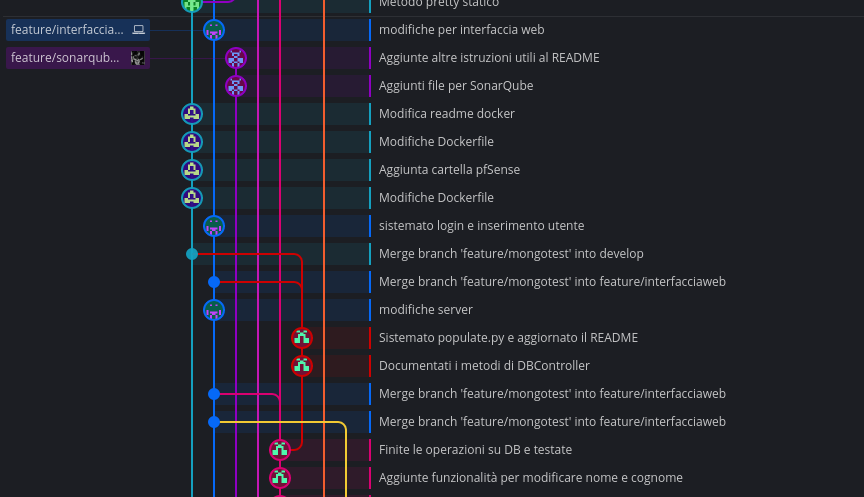
\includegraphics[width=\textwidth]{img/branches.png}\\
		\caption[Albero dei branch da Gitkraken]{Visione generale dell'albero dei branch in un momento casuale da Gitkraken}
		\label{fig:butterfly}
	\end{figure}

	\subsubsection{Aggiornamento della repository}

	Per aggiornare la repository remota con i cambiamenti effettuati nella workcopy locale, la prassi da seguire è la seguente:
	\begin{itemize}
		\item Controllare di trovarsi nel branch corretto con il comando:
			\begin{quote}
				\texttt{\$\ git branch}
			\end{quote}
			In caso negativo, dare il comando \texttt{git checkout nomebranch} per spostarsi nel branch corretto prima di procedere.
		\item Aggiornare la workcopy locale con eventuali cambiamenti presenti nella repository remota:
			\begin{quote}
				\texttt{\$\ git pull}
			\end{quote}
		\begin{itemize}
			\item In caso di conflitti, dare la sequenza di comandi che segue per risolverli senza dover effettuare un commit
				dedicato solo al merge:
				\begin{quote}
					\texttt{\$\ git stash}\par
					\texttt{\$\ git pull}\par
					\texttt{\$\ git stash pop}\par				
				\end{quote}
				A questo punto, si potrebbero avere dei conflitti marcati opportunamente da Git, oppure avere la copia aggiornata
				con le proprie modifiche applicate.
		\end{itemize} 
		\item Aggiungere i file allo ``stage'' relativi a una specifica modifica con il comando (è possibile usare * come wildcard
			per aggiungere più file contemporaneamente):
			\begin{quote}
				\texttt{\$\ git add [nome-file1] [nome-file2] \dots}
			\end{quote}
		\item Fare il commit e riassumere i cambiamenti apportati:
		\begin{quote}
			\texttt{\$\ git commit -m "Cambiamenti apportati"}
		\end{quote}
		\item Effettuare il push per pubblicare le modifiche locali nella repository remota:
		\begin{quote}
			\texttt{\$\ git push}
		\end{quote}
	\end{itemize}


	\subsection{Verifica}\label{Verifica}

		\subsubsection{Scopo}
		Questa sezione vuole descrivere come eseguiamo la fase di verifica, per capire se i prodotti e i processi sono conformi a quanto ci attendiamo.
		La fase di verifica serve per stabilire se è opportuno o meno procedere alla fase successiva del progetto, se ciò non fosse possibile sarà necessario il
		ritorno ad una fase stabile del progetto per poi ripartire da lì, prendendo in considerazione i risultati della precedente verifica.

		%\subsubsection{Aspettative} %da mettere nel PdQ

		\subsubsection{Descrizione}
		Ogni processo e prodotto deve essere valutato in modo quantificabile attraverso metriche apposite, quando possibile, e stabilendo il risultato che si vuole
		raggiungere.

		Come indicato dal \gloss{Ciclo di Deming} nel \Doc{\PdQv}, nel momento in cui tale risultato sarà raggiunto, se esso non è il migliore,
		servirà come ``base'' per alzare il livello di qualità di quel processo o prodotto.

		I risultati ottenuti nella fase di verifica sono riportati nel \PdQ: in questo modo, confrontandoli con gli esiti attesi,
		è possibile valutare un miglioramento per i vari processi e prodotti sempre nel \PdQ.

		\subsubsection{Walkthrough e Inspection}
		Due modi di effettuare la verifica sono attraverso \gloss{Walkthrough} e Inspection.
		Li adotteremo entrambi, ma non contemporaneamente, per i vantaggi che comporta ogni metodo.

			\paragraph{Walkthrough}
			Metodo di verifica che effettua un controllo ad ampio spettro senza l’assunzione di presupposti. Dato che per mettere in atto tale metodo ci
			si deve dividere in gruppi dove ognuno ha un ruolo ben distinto, Walkthrough è ideale per le verifiche effettuate all'inizio dei vari periodi,
			dove i membri del team di sviluppo non possiedono le conoscenze adeguate per una verifica efficiente.

			Walkthrough possiede delle fasi ben specifiche:

			\begin{enumerate}
				\item \textbf{Pianificazione}: viene pianificato in gruppo come effettuare la verifica dei prodotti.
				\item \textbf{Lettura}: viene effettuata la lettura del prodotto.
				\item \textbf{Discussione}: vengono discusse le possibili correzioni.
				\item \textbf{Correzione di difetti}: si attuano i risultati ottenuti dalla fase di discussione.
			\end{enumerate}

			\paragraph{Inspection}
			Metodo di verifica dove si esegue una lettura mirata dei prodotti, frutto di un'analisi dei risultati sei precedenti test.
			Questo metodo dunque, a differenza di Walkthrough, prevede l'esecuzione con dei presupposti.
	
			Le fasi di Inspection sono:
	
			\begin{enumerate}
				\item \textbf{Pianificazione}: viene sempre pianificato in gruppo come effettuare la pianificazione.
				\item \textbf{Definizione di una lista di controllo}: dato che le parti da verificare sono specificate, queste possono essere
				riportate in una lista in modo da velocizzare il processo di verifica.
				\item \textbf{Correzione dei difetti}: attuazione dei punti della lista di controllo.
			\end{enumerate}
	
			Per la natura di Inspection, questa non può essere applicata fin dall'inizio, dunque nel momento in cui si presentano nuove tipologie di
			prodotti e processi da verificare viene effettuato Walkthrough; nel momento in cui il metodo di verifica è ben consolidato da tutti noi,
			si passa ad effettuare verifica secondo Inspection.	

		\subsubsection{The Twelve-Factor App}
		\gloss{The Twelve-Factor App} è una serie di dodici regole destinate a chi vuole sviluppare \gloss{software-as-a-service} (SaaS). Sono utili per verificare in corso d'opera la qualità del progetto, valutando quali punti riesce a rispettare l'applicazione.
		
		I suoi principi sono:
		
		\begin{enumerate}
			\item \textbf{\gloss{Codebase}}: deve essere presente una sola codebase versionata da un \gloss{Version Control System} (VCS) come \gloss{GitLAb} da cui
			possono derivare diversi \gloss{deploy}.
			\item \textbf{Dipendenze}: le librerie usate dal codice devono essere presenti nella directory della singola applicazione e non attive a livello di \gloss{sistema}. In questo modo l'applicazione è il meno dipendente possibile dal sistema di esecuzione.
			\item \textbf{Configurazione}: i parametri di configurazione dell'applicazione devono essere completamente separati dalla sua implementazione.
			\item \textbf{Backing Service}: l'applicazione non deve far distinzione tra funzionalità uguali usate in locale o remoto.
			\item \textbf{Build, release, esecuzione}: bisogna separare in modo netto la fase di build, quella di deploy e quella esecuzione, usando \gloss{tool} differenti e diverse repository per salvare i risultati delle varie fasi.
			\item \textbf{Processi}: l'esecuzione dell'applicazione deve essere vista come l'insieme di uno o più processi che restituiscono un risultato. Questi sono di tipo \gloss{stateless}.
			\item \textbf{\gloss{Binding} delle Porte}: l'applicazione è completamente contenuta in se stessa e non fa affidamento ad un altro servizio nell'ambiente di esecuzione. Effettua invece il binding delle porte diventando un servizio per le richieste esterne.
			\item \textbf{Concorrenza}: sviluppare i processi in modo tale che possano lavorare su un sistema decentralizzato.
			\item \textbf{Rilasciabilità}: i processi dell'applicazione devono poter essere avviati e fermati quando se ne ha bisogno senza passaggi bruschi.
			\item \textbf{Parità tra sviluppo e produzione}: deve esserci meno differenza possibile tra lo stato di sviluppo e quello di produzione. Questo si ottiene facendo un rilascio continuo del prodotto.
			\item \textbf{Log}: l'applicazione dovrebbe poter offrire un sistema di login.
			\item \textbf{Processi di Amministrazione}: porre attenzione a quei processi che devono essere eseguiti una tantum dagli sviluppatori ad esempio. Questi processi devono poter essere accessibili solo ad alcuni e indicati in una specifica release.
		\end{enumerate}
		
		In accordo col cliente \II, non tutti i punti di Twelve-Factor App possono essere rispettati. In particolare non è richiesto il soddisfacimento del punto 12, mentre il punto 11 è lasciato al fornitore come opzionale.
		
		
		\subsubsection{Analisi statica}\label{AnalisiStatica}
		L'analisi statica verifica solo i prodotti che non sono o che non possono essere eseguiti, come i documenti.

			\paragraph{Analisi dei documenti}
			L'analisi statica per i documenti si limita a valutare come e con che contenuti questi vengono scritti.
			Per l'analisi dei documenti vengono utilizzate:

			\begin{itemize}
				\item MPD001
				\item MPD002
			\end{itemize}

			\paragraph{Analisi dei processi}
			Per analizzare i processi usiamo gli standard sopra elencati. Ad ogni fase del processo, verranno valutati gli attributi richiesti secondo
			l'ISO 15504, in che misura questi sono stati rispettati e in che fase del Ciclo di Deming il processo si trova.
			Per l'analisi dei processi vengono utilizzate:

			\begin{itemize}
				\item MPR001 Varianza della pianificazione
				\item MPR002 Varianza dei costi
				\item MPR004 Frequenza commit nella repository
				\item MPR009 Frequenza controllo prodotti
				% \item \textbf{MPR010 Norme di progetto non seguite}
			\end{itemize}


			\paragraph{Metriche}
			La denominazione delle metriche è descritta in \S\ref{Classificazione metriche}.
		
			\subparagraph{MPR009 Frequenza controllo prodotti}
			I documenti e i prodotti software hanno bisogno di una verifica frequente, commisurata in base al numero di modifiche che vengono apportate.
		
			Chi esegue la modifica deve controllare ciò che ha fatto prima di poterla ufficializzare, mentre la verifica fatta dal \Ver\ deve essere
			fatta solo nel momento in cui è stato raggiunto un numero significativo di modifiche, per evitare di spendere troppe risorse in questa fase.
		
			\[\dfrac{\sum_{i=1}^{n} x_i}{n} \qquad x_i=\text{numero di modifiche effettuate prima della i-esima verifica.}\]
		
			\textbf{Metrica}: media del numero massimo di modifiche apportate ai prodotti prima che ricevano una verifica dal parte del \Ver.

		
		
		\subsubsection{Analisi dinamica}\label{AnalisiDinamica} %TODO
		L'analisi dinamica valuta il comportamento dei prodotti in esecuzione, verificando se restituiscono i risultati attesi e se operano nel modo stabilito.
		Vengono presi in esame i prodotti software e i processi.
		%Parlare dei test..
		
			\paragraph{Procedure} %TODO: prendere spunto da 3.2.6.2.4 Breaking Bug RA
			%Ogni test deve essere ripetibile.. ogni test vengano segnati i seguenti riferimenti:
			\begin{itemize}
				\item \textbf{Ambiente di sviluppo}:
				\item \textbf{Stato iniziale}:
				\item \textbf{Input}: inserito.
				\item \textbf{Output}: atteso.
				\item \textbf{Notifica risultato}:
			\end{itemize}
		
			%RICONTROLLARE BENE MODELLO A V PER I PROSSIMI PARAGRAFI DI TEST
			
			\paragraph{Test di sistema} %TODO
			%Contenuto
			
			\paragraph{Test d'integrazione} %TODO
			%Contenuto
			
			\paragraph{Test di unità} %TODO
			%Contenuto
			
			\paragraph{Test di regressione} %TODO
			%Contenuto
			
			\paragraph{Test di accettazione} %TODO
			%Contenuto
		
		
		\subsubsection{Tipologie e trattamento delle anomalie riscontrate}\label{TrattamentoAnomalie} %TODO
		%Anomalie dovute al mancato rispetto dei valori di riferimento stabiliti per le metriche applicate... e Anomalie dovute al mancato superamento dei test pianificati.....
		